\documentclass[conference]{IEEEtran}

\usepackage{cite}
\usepackage{graphicx}
\usepackage{amsmath}
\usepackage{amssymb}
\usepackage{booktabs}
\usepackage{array}
\usepackage{multirow}
\usepackage{siunitx}
\usepackage{url}
\usepackage[table]{xcolor}
\usepackage[caption=false,font=footnotesize]{subfig}

\sisetup{
  group-separator={,},
  group-minimum-digits=4,
  table-number-alignment=center,
  input-symbols = {()},
  table-align-text-post = false
}

\begin{document}
% Long two-column preprint with many floats: avoid stretched inter-paragraph gaps.
\raggedbottom

\title{Does Gait Timing Knowledge Transfer Across Neurological Conditions? A Zero-Shot Benchmark with SHAP-Based Transfer Diagnostics}

\author{
\IEEEauthorblockN{Ahmad Shahmeer}
\IEEEauthorblockA{School of Electrical Engineering\\
and Computer Science (SEECS)\\
National University of Sciences\\
and Technology (NUST)\\
Islamabad, Pakistan\\
ahmadshahmeer.work@gmail.com}
\and
\IEEEauthorblockN{Ali Aqdas}
\IEEEauthorblockA{School of Electrical Engineering\\
and Computer Science (SEECS)\\
National University of Sciences\\
and Technology (NUST)\\
Islamabad, Pakistan\\
info@aliaqdas.dev}
}

\maketitle

\begin{abstract}
We study whether an abnormal-versus-control gait timing boundary learned for one neurological condition remains useful when it is applied, without retraining, to another. Using the PhysioNet gait database in neurodegenerative disease, we build a leakage-controlled benchmark of all six directed transfers among Parkinson's disease (PD), Huntington's disease (HD), and amyotrophic lateral sclerosis (ALS), with 63 subjects, 13{,}765 stride rows, and 14 engineered timing features. Within-condition performance is estimated by nested subject-level leave-one-subject-out validation. Each transfer model is selected and refitted on its complete source pool and evaluated once on the target, and the healthy controls are split into disjoint source and target pools. Within condition, the leading models reach subject-level macro-$F_1$ of 0.9042 for PD, 0.9571 for HD, and 1.0000 for ALS. Averaged over seven classifier families, matched degradation is positive in all six directions, although seven of the 42 classifier-direction pairs exceed their matched within-source baseline. The best model in each direction can only be identified after observing target labels, so these leaders describe the best observed outcome and not an operational selection rule. SHAP reliance-shift and permutation diagnostics place the largest aggregate burden on variability and raw timing features. The results depend strongly on the control partition: one alternate balanced partition reverses four of the six direction-level signs. Gait timing transfer across these conditions is measurable but degraded, asymmetric, and sensitive to which healthy subjects are used.
\end{abstract}

\begin{IEEEkeywords}
gait analysis, neurodegenerative disease, zero-shot transfer, domain shift, subject-level evaluation, SHAP, Parkinson's disease, Huntington's disease, amyotrophic lateral sclerosis
\end{IEEEkeywords}

\section{Introduction}
\label{sec:intro}
Parkinson's disease (PD), Huntington's disease (HD), and amyotrophic lateral sclerosis (ALS) all impair walking, but through different disease processes. Stride timing becomes more variable in PD and HD, the long-range correlation of the stride interval series is reduced in HD, and gait rhythm changes in ALS as motor neurons are lost \cite{hausdorff1997fractal,hausdorff1998variability,hausdorff2000als}. Stride timing is inexpensive to record and compact to represent, and it can be compared across disorders that share locomotor impairment without sharing a pathology. For these reasons it is a common input for automated gait assessment.

Machine learning studies on these cohorts are almost always evaluated within a single condition. A reported accuracy then shows that a disease-versus-control boundary exists in that cohort, but it says little about whether the boundary reflects gait abnormality more generally. If a boundary learned on PD keeps some predictive value when it is applied without retraining to HD or ALS, then part of what the model learned is not specific to PD. If it does not, the boundary may depend on source-specific disease or cohort structure. The question is most relevant where labelled data are scarce, which is the usual situation for HD and ALS.

Answering it correctly depends on how the healthy controls are handled. Every abnormal-versus-control task needs controls on both sides, and public gait cohorts are small enough that the same healthy subjects would normally appear in the source training pool and in the target evaluation pool. A transferred model could then score well by recognising healthy gait it had already seen, while failing on the disease side it was meant to generalise to. We therefore divide the healthy subjects once, before any task is defined, into two disjoint pools: one used only for training and one used only for evaluation (Fig.~\ref{fig:protocol}). Both the disease cohort and the healthy pool change when a model is transferred, so the setting is zero-shot for both classes.

\begin{figure*}[t]
\centering
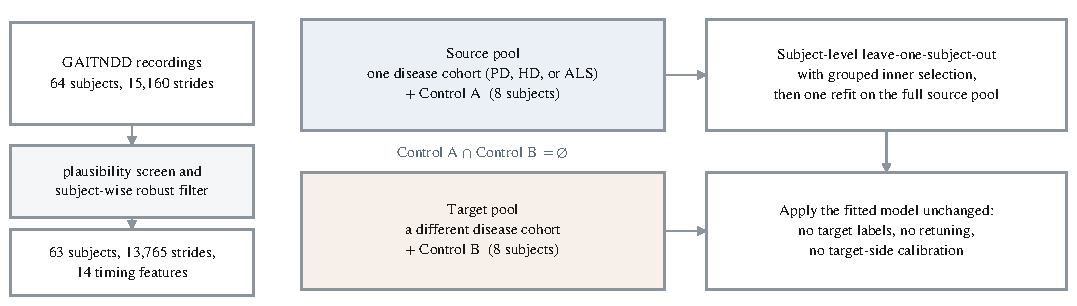
\includegraphics[width=\textwidth]{figures/arxiv/protocol.pdf}
\caption{Cohort accounting and the control-disjoint transfer design. A source model is selected and refitted using one disease cohort together with Control~A, then applied unchanged to a different disease cohort scored against Control~B. Because the two control pools are disjoint, a transfer score cannot be inflated by re-recognising healthy subjects seen during training.}
\label{fig:protocol}
\end{figure*}

A transfer score on its own cannot show why a model lost accuracy. The model may have started to rely on different features, it may be sensitive to small changes in its inputs, or its result may depend on which healthy subjects were available. We therefore pair the benchmark with three diagnostics: a SHAP-based measure of how far each model's reliance moves between source and target, stride-level stress tests of the fitted models, and a repetition of the complete protocol under alternate balanced control partitions. The diagnostics describe model behaviour, and none of them is interpreted as evidence about disease mechanism.

This paper makes four contributions.
\begin{itemize}
\item A leakage-controlled benchmark of all six directed zero-shot transfers among PD, HD, and ALS on GAITNDD, with subject-level endpoints, nested within-condition estimation, disjoint healthy control pools, and full-source refits evaluated once on the target.
\item A matched-degradation analysis that compares each classifier family with its own within-condition estimate and keeps classifier averages separate from retrospectively identified direction leaders.
\item A reliance-shift diagnostic whose family-level aggregation does not let opposing feature movements cancel, reported together with stride-level robustness and permutation analyses.
\item A control-partition sensitivity analysis that shows how strongly the conclusions depend on the assignment of eight healthy subjects per pool, with the code, manifests, and result files released publicly \cite{gait-transfer-repo}.
\end{itemize}

Within-condition subject-level baselines are strong. Averaged over seven families every direction degrades under transfer, while seven individual classifier-direction pairs exceed their matched baselines. The reliance-shift and permutation diagnostics place the largest aggregate burden on variability and raw timing. One alternate balanced partition reverses four of the six direction signs, mainly because the within-condition tasks become harder under it. Transfer in this cohort is measurable, but it is degraded, asymmetric, and dependent on the control partition.

The rest of the paper is organised as follows. Section~\ref{sec:related} reviews related work. Section~\ref{sec:data} describes the dataset, preprocessing, control partition, and features. Section~\ref{sec:method} defines the learning, transfer, and diagnostic methods, and Section~\ref{sec:setup} gives the grids, inference procedures, diagnostic settings, and reproducibility measures. Section~\ref{sec:results} presents the results, Section~\ref{sec:discussion} discusses their interpretation and limitations, and Section~\ref{sec:conclusion} concludes.

\section{Related Work}
\label{sec:related}

\subsection{Classification on GAITNDD}
Studies that use this database almost always train and evaluate within one observed label space. Yan et al. \cite{yan2020tma} embedded gait fluctuation series in a phase space, extracted topological signatures, and classified each disease against healthy controls with a random forest under leave-one-out evaluation, reporting strong separability for all three cohorts. Erda\c{s} and S\"umer \cite{erdas2024qr} converted the same recordings into QR-like images and trained convolutional networks under ten-fold cross-validation, both for disease-versus-control tasks and for classification over the pooled label space. Both studies establish that these recordings carry discriminative structure. Neither evaluates cross-condition transfer in which the healthy subjects used for source training are disjoint from those used for target scoring, which is the setting studied here.

\subsection{Gait-Based Assessment Beyond Binary Diagnosis}
Other work keeps the in-domain framing while changing the clinical target. Khera et al. \cite{khera2025severity} treat neurodegenerative gait assessment as a hierarchical decision-tree problem that first separates disease from control and then refines severity, which keeps the model interpretable but still operates inside one observed cohort. PD-focused studies such as Mittal et al. \cite{mittal2025pd} and Navita et al. \cite{navita2025force} address diagnosis and severity estimation from timing-derived or force-derived gait features within a single disease population. A recent survey of artificial intelligence for gait-based neurodegenerative diagnosis identifies generalisation across cohorts and conditions as an open problem \cite{rao2024gaitsurvey}. Across these studies the dominant question is how well a model discriminates or stages patients within the population it was trained on.

\subsection{Explainability in Gait Analysis}
Attribution methods are increasingly used to interpret gait models. SHAP provides a general additive framework for attributing a prediction to input features \cite{lundberg2017shap}. A systematic review of explainable methods in gait analysis, covering SHAP, LIME, gradient-based saliency, and attention mechanisms, reports that attribution is used predominantly to explain a fitted model within its own evaluation domain \cite{xiang2025xai}. Our use of SHAP is narrower. We do not interpret attribution patterns as evidence about disease mechanism. We measure how far the reliance profile of a fixed source model moves when that model is applied to a condition it was not trained on.

\subsection{Transfer Learning and Domain Shift}
The transfer learning and domain generalisation literature describes the setting studied here. Source and target share a binary abnormal-versus-control task but differ in disease population and in healthy-control membership, which is the domain-shift regime surveyed by Pan and Yang \cite{pan2010transfer}. Because no target label, calibration set, or tuning signal is available, the model has to generalise from source data alone, as in domain generalisation \cite{zhou2021dgsurvey}. We do not assume that the shift affects only the input distribution. The condition-specific relation between gait timing and the abnormal label may itself change between source and target.

\subsection{Positioning}
The protocols in Table~\ref{tab:prior-work} differ too much for a direct performance comparison, so we present this work as a benchmark with diagnostics and not as a new classifier. To our knowledge, the six directed disease-to-disease transfers have not been reported for GAITNDD under subject-level evaluation with disjoint control pools, and no gait study has combined such a benchmark with reliance-shift diagnosis, robustness stress tests, and control-partition sensitivity.

\begin{table*}[t]
\caption{Positioning of this study relative to related work on gait classification, explainability, and transfer.}
\label{tab:prior-work}
\centering
\footnotesize
\begingroup
\setlength{\tabcolsep}{3pt}
\renewcommand{\arraystretch}{1.08}
\begin{tabular}{>{\raggedright\arraybackslash}p{0.14\linewidth}>{\raggedright\arraybackslash}p{0.21\linewidth}>{\raggedright\arraybackslash}p{0.15\linewidth}>{\raggedright\arraybackslash}p{0.13\linewidth}>{\raggedright\arraybackslash}p{0.12\linewidth}>{\raggedright\arraybackslash}p{0.16\linewidth}}
\toprule
Study or theme & Data and task & Validation & Transfer setting & Interpretability & Relation to this study \\
\midrule
Yan et al. \cite{yan2020tma} & GAITNDD disease-versus-control classification from topological fluctuation features & Leave-one-out within each binary task & In-domain & Engineered structural features & Same dataset; no cross-condition transfer \\
Erda\c{s} and S\"umer \cite{erdas2024qr} & GAITNDD CNN classification from QR-like images, binary and pooled label space & Ten-fold cross-validation & In-domain & Not reported & Same dataset; no control-disjoint transfer \\
Khera et al. \cite{khera2025severity} & Hierarchical disease and severity assessment from gait & In-domain hierarchical classification & In-domain & Interpretable tree structure & Staging within one cohort, not transfer \\
Mittal et al. \cite{mittal2025pd}, Navita et al. \cite{navita2025force} & PD diagnosis and severity from timing or force features & Single-disease evaluation & In-domain & Feature selection within PD & Adjacent gait machine learning \\
Xiang et al. \cite{xiang2025xai} & Review of explainable methods in gait analysis & Review & Not applicable & Central topic & Attribution mainly within the fitted domain \\
Transfer and domain shift \cite{pan2010transfer,zhou2021dgsurvey} & Transfer learning and generalisation to unseen domains & Methodological surveys & Source-only generalisation & Not the focus & Vocabulary for the transfer setting \\
This study & GAITNDD abnormal-versus-control transfer among PD, HD, and ALS & Subject-level LOSO with grouped inner selection & Six directed transfers with disjoint control pools & SHAP reliance shift & Control-disjoint transfer with diagnostics and partition sensitivity \\
\bottomrule
\end{tabular}
\endgroup
\end{table*}

\section{Dataset and Preprocessing}
\label{sec:data}

\subsection{PhysioNet Gait Database in Neurodegenerative Disease}
We use the PhysioNet gait database in neurodegenerative disease (GAITNDD) \cite{physionet_gaitndd}, distributed through PhysioNet \cite{goldberger2000physiobank}. The release provides one stride timing series per subject, derived from force signals recorded under each foot during walking. Each row contains the elapsed time and 12 temporal gait variables: left and right stride, swing, and stance durations, left and right swing and stance percentages, and double-support duration and percentage. The same recordings underlie the original studies of stride variability and fractal gait dynamics in PD, HD, and ALS \cite{hausdorff1997fractal,hausdorff1998variability,hausdorff2000als}. We keep this timing representation, treat each stride as a row, and retain subject identifiers for grouped validation, subject-level aggregation, and transfer evaluation. The elapsed time is discarded.

The raw release covers 64 subjects and 15{,}160 stride rows: 15 PD subjects, 20 HD subjects, 13 ALS subjects, and 16 healthy controls.

\subsection{Cleaning and Exclusions}
Two filtering stages are applied before any task is defined. The first is a plausibility screen. A row is removed if any stride, swing, or stance duration is non-positive, if double-support time is negative, if either stride duration exceeds 3.0~s, or if any percentage lies outside $[0,100]$. Stride durations above 3.0~s mark pauses or sensor failures rather than walking. This screen leaves 14{,}751 rows and removes every stride of one HD subject, so the usable HD cohort falls from 20 to 19 subjects.

The second stage is a subject-wise robust filter on left stride time, right stride time, and double-support time. For each subject and each of these variables, strides are retained if they fall within three scaled median absolute deviations of that subject's median, where the scaled deviation is 1.4826 times the median absolute deviation. The filter is intended to remove turning, pausing, and acceleration artifacts that would otherwise distort the variability and fluctuation descriptors. It is skipped for any subject whom it would leave with fewer than 100 strides, which happened for one ALS subject. This stage removes a further 986 rows. Table~\ref{tab:cohort} summarises the resulting cohort.

\begin{table}[t]
\caption{Cohort after each preprocessing stage and final composition of the analysed matrix.}
\label{tab:cohort}
\centering
\footnotesize
\setlength{\tabcolsep}{4pt}
\begin{tabular}{lrr}
\toprule
Stage or group & Subjects & Stride rows \\
\midrule
Raw release & 64 & 15{,}160 \\
After plausibility screen & 63 & 14{,}751 \\
After subject-wise robust filter & 63 & 13{,}765 \\
\midrule
PD & 15 & 3{,}414 \\
HD & 19 & 4{,}280 \\
ALS & 13 & 2{,}285 \\
Healthy controls & 16 & 3{,}786 \\
\quad Control~A (source pools) & 8 & 1{,}934 \\
\quad Control~B (target pools) & 8 & 1{,}852 \\
\bottomrule
\end{tabular}
\end{table}

\subsection{Disjoint Control Partition}
\label{sec:data-partition}
The 16 healthy controls are divided once into two groups of eight before any model is fitted. Control~A contains control subjects 1, 2, 3, 4, 6, 7, 11, and 16, and Control~B contains subjects 5, 8, 9, 10, 12, 13, 14, and 15. The split is one of the partitions with the smallest standardised difference between the groups in mean age and mean gait speed, among those that place one male subject in each group. The groups differ by 0.125 years in mean age (39.375 against 39.25) and by 0.00375~m/s in mean gait speed (1.3525 against 1.35625). This balancing makes the two healthy pools comparable to each other. It does not make either pool demographically comparable to the disease cohorts, and we make no such claim.

Control~A supplies the healthy strides for every source pool and for every full-source transfer model. Control~B is used only for target-side evaluation. As a result, no healthy subject appears in both the training and the evaluation of any transfer. Without this separation, a transferred model could score well by recognising healthy subjects it had already seen, even if its disease-side boundary failed to generalise.

\subsection{Feature Representation}
\label{sec:data-features}
The analysed matrix contains 14 engineered features in five families, listed in Table~\ref{tab:features}. Seven are raw timing durations and three are phase percentages. The asymmetry index is the absolute difference between left and right stride time divided by their mean. The two variability descriptors are the coefficients of variation of left stride time and left swing time, and the fractal descriptor is the detrended fluctuation exponent of the stride-time series. The variability and fractal descriptors are computed once per subject over the retained strides and repeated on every row of that subject.

\begin{table}[t]
\caption{Engineered features with the identifiers used in the figures. Features marked $\dagger$ are computed once per subject and repeated on each of that subject's strides; all others are computed per stride.}
\label{tab:features}
\centering
\footnotesize
\setlength{\tabcolsep}{3pt}
\begin{tabular}{lll}
\toprule
Identifier & Description & Family \\
\midrule
\texttt{left\_stride\_s} & Left stride time & raw timing \\
\texttt{right\_stride\_s} & Right stride time & raw timing \\
\texttt{left\_swing\_s} & Left swing time & raw timing \\
\texttt{right\_swing\_s} & Right swing time & raw timing \\
\texttt{left\_stance\_s} & Left stance time & raw timing \\
\texttt{right\_stance\_s} & Right stance time & raw timing \\
\texttt{double\_support\_s} & Double-support time & raw timing \\
\texttt{left\_swing\_pct} & Left swing percentage & phase percentage \\
\texttt{right\_swing\_pct} & Right swing percentage & phase percentage \\
\texttt{double\_support\_pct} & Double-support \% & phase percentage \\
\texttt{asymmetry\_index} & Stride-time asymmetry & asymmetry \\
\texttt{cv\_stride}$^\dagger$ & CV of left stride time & variability \\
\texttt{cv\_swing}$^\dagger$ & CV of left swing time & variability \\
\texttt{dfa\_alpha\_stride}$^\dagger$ & Fluctuation exponent & fractal \\
\bottomrule
\end{tabular}
\end{table}


We exclude the left and right stance percentages, which are exact complements of the swing percentages, and a signed stride asymmetry term that added little beyond the absolute index. The representation is compact and fully traceable to the timing series. It is not a complete clinical description of gait.

Three properties limit how the features can be interpreted. Within the raw timing family the variables are mechanically linked, since stride duration is the sum of its stance and swing components, so single-variable readings inside that family should be treated with caution. The phase percentages are compositional and remain partly constrained even after the exact complements are removed, so they are better read as a family than as independent clinical axes. The subject-level descriptors summarise longer-horizon structure but are attached to individual strides. The fluctuation exponent in particular is estimated from a stride series that contains gaps where filtered rows were removed, using log-spaced window sizes from 4 strides to a quarter of the series length. It is a pragmatic descriptor and should not be read as a complete fractal biomarker.

\section{Methodology}
\label{sec:method}

\subsection{Task Formulation and Subject-Level Aggregation}
We define three binary abnormal-versus-control tasks, one per source condition, instead of a single classifier of disease identity. In each task the positive class contains all retained strides of one disease cohort and the negative class contains all retained strides of Control~A. The three source pools are PD with Control~A (23 subjects, 5{,}348 strides), HD with Control~A (27 subjects, 6{,}214 strides), and ALS with Control~A (21 subjects, 4{,}219 strides). A positive prediction in the HD task means ``stride from an HD subject'', not ``stride from any neurological patient''.

Stride rows are the unit of model input, but they are not independent observations, since each subject contributes many correlated strides. Evaluation is carried out at the subject level. For subject $s$ with $n_s$ retained strides and predicted disease probabilities $\hat{p}_{si}$, we compute
\begin{equation}
\hat{p}_s = \frac{1}{n_s}\sum_{i=1}^{n_s}\hat{p}_{si},
\qquad
\hat{y}_s = \mathbb{I}\!\left[\hat{p}_s \ge 0.5\right],
\label{eq:subject-aggregation}
\end{equation}
and report subject-level macro-$F_1$ as the primary endpoint. Stride-level macro-$F_1$ is kept as a descriptive companion. Evaluating at the subject level prevents subjects with long recordings from dominating the result.

\subsection{Within-Condition Estimation}
\label{sec:method-within}
Within-condition performance is estimated by outer leave-one-subject-out cross-validation (LOSO). On each outer split, all strides of one subject are held out, and the remaining subjects form the outer training pool. Candidate selection takes place entirely inside that pool through a grouped inner LOSO loop, so the held-out subject is never seen during tuning. The candidate space is the product of each family's hyperparameter grid with its permitted imbalance strategies.

Inner scores are pooled before candidates are compared. For each candidate, the pipeline is fitted on the inner training subjects and used to predict the inner held-out subject, the predictions are concatenated across all inner held-out subjects, and the pooled predictions are scored at the subject level. Pooling prevents a single small inner fold from deciding the selection, and keeping selection inside the outer training pool prevents selection bias from entering the reported estimate \cite{cawley2010overfitting}. Candidates are ranked by pooled subject-level macro-$F_1$, with ties broken first by lower pooled subject-level log loss and then by a deterministic ordering of the candidate definition. The winning candidate is refitted on the full outer training pool and evaluated on the outer held-out subject.

The outer-LOSO subject-level macro-$F_1$ of each family is the within-condition estimate for that family. It also serves as the family's matched baseline in the transfer analysis.

\subsection{Pipelines and Imbalance Handling}
We compare seven classifier families: random forest (RF), $k$-nearest neighbours (KNN), a support vector machine with an RBF kernel (SVM), a decision tree (DT), quadratic discriminant analysis (QDA), XGBoost, and LightGBM. The grids are listed in Section~\ref{sec:setup-grids}.

Each candidate uses one of three imbalance strategies. The first applies no resampling and no weighting. The second applies balanced class or sample weights where the estimator supports them. The third inserts SMOTE \cite{chawla2002smote} into the pipeline, so that synthetic samples are generated from the training portion of each split only. Control~A is the minority class in every source pool, because eight healthy subjects are paired with 13 to 19 disease subjects, so SMOTE creates synthetic healthy strides, not disease strides.

Scaling depends on the family and the strategy. SVM and KNN always include a robust scaler, because kernel and distance computations are sensitive to unequal feature scales. Every SMOTE pipeline is also scaled before interpolation, whatever the family, so that synthetic samples are generated in a scaled space. Tree-based models and QDA otherwise use the unscaled engineered features. All stochastic components use a fixed seed.

\subsection{Zero-Shot Transfer Protocol}
\label{sec:method-transfer}
The transfer analysis asks whether a boundary learned for one condition can be applied directly to another condition without any target-side retraining, tuning, or calibration. We evaluate all six directed transfers: PD~$\rightarrow$~HD, HD~$\rightarrow$~PD, PD~$\rightarrow$~ALS, ALS~$\rightarrow$~PD, HD~$\rightarrow$~ALS, and ALS~$\rightarrow$~HD. The source pool is always a disease cohort with Control~A, and the target pool is always a different disease cohort with Control~B. Target pools contain between 21 and 27 subjects.

The transfer model does not reuse settings from the outer folds. After the within-condition analysis, each family receives one further grouped selection on its complete source pool, using the same candidate space, objective, and tie-break rule, and the selected candidate is refitted on that pool. This full-source model is applied once, unchanged, to the target pool. No target label, hyperparameter, threshold, or calibration set is used at any stage.

We summarise transfer cost by the matched degradation
\begin{equation}
\Delta F_1 = F_{1,\mathrm{subject}}^{\mathrm{within}} - F_{1,\mathrm{subject}}^{\mathrm{cross}},
\label{eq:matched-degradation}
\end{equation}
where both terms refer to the same classifier family: $F_{1,\mathrm{subject}}^{\mathrm{within}}$ is that family's outer-LOSO estimate on the source task, and $F_{1,\mathrm{subject}}^{\mathrm{cross}}$ is the score of its full-source model on the target pool. A positive value means the model did worse on the unseen condition than within its own condition, and a negative value means it did better. The comparison is never made against the leading classifier of the source condition.

Each direction is summarised in two ways. The classifier average is the unweighted mean over the seven families. It is a descriptive summary of this benchmark and not an estimate over classifiers in general. The retrospective direction leader is the family with the highest cross-condition subject-level macro-$F_1$ in that direction. Because it is identified after the target labels have been scored, it shows the best observed outcome among the evaluated families and does not define a model-selection rule.

\subsection{Reliance-Shift Diagnostic}
\label{sec:method-shap}
A transfer score shows whether a model remained useful but not which features it began to use differently. We measure this with SHAP \cite{lundberg2017shap}. For each full-source model, SHAP values are computed on the source pool on which the model was fitted and on the target pool, and the two are compared feature by feature. For feature $j$, let $\overline{|\phi^{\mathrm{within}}_j|}$ and $\overline{|\phi^{\mathrm{cross}}_j|}$ be the mean absolute SHAP values on the source and target pools. The raw shift is
\begin{equation}
\delta_j = \left|\;\overline{\left|\phi^{\mathrm{within}}_j\right|} - \overline{\left|\phi^{\mathrm{cross}}_j\right|}\;\right|,
\label{eq:delta-j-raw}
\end{equation}
where taking absolute values first prevents positive and negative contributions from cancelling. A raw shift is hard to compare across features with very different reliance levels, so we also use a normalised shift,
\begin{equation}
\begin{split}
\widetilde{\delta}_j = \min\!\left(\frac{\delta_j}{\max\!\left(\overline{\left|\phi^{\mathrm{within}}_j\right|},\, \epsilon\right)},\; C\right),\\
\epsilon = 10^{-10},\quad C = 10,
\end{split}
\label{eq:delta-j-normalized}
\end{equation}
where the floor $\epsilon$ avoids division by zero and the cap $C$ stops a feature that the source model barely used from dominating the ranking. A feature is flagged as emerged when its within-source reliance is below $10^{-3}$ and its shift is positive.

Feature shifts are also aggregated over the five feature families. For family $\mathcal{F}$ we use the total movement
\begin{equation}
M_{\mathcal{F}} = \sum_{j \in \mathcal{F}} \left|\;\overline{\left|\phi^{\mathrm{within}}_j\right|} - \overline{\left|\phi^{\mathrm{cross}}_j\right|}\;\right|,
\label{eq:total-movement}
\end{equation}
which sums absolute feature-level changes. We prefer it to the net shift $\bigl|\sum_{j\in\mathcal{F}} \overline{|\phi^{\mathrm{within}}_j|} - \sum_{j\in\mathcal{F}} \overline{|\phi^{\mathrm{cross}}_j|}\bigr|$, which allows a rise in one feature to cancel a fall in another feature of the same family.

The explainer follows the model family. RF and DT use the path-dependent tree explainer, whose output is already on the probability scale. XGBoost and LightGBM use the interventional tree explainer with probability output, so that their attributions share that scale. SVM, QDA, and KNN use the kernel explainer on the probability output of the complete fitted pipeline, which keeps attributions in the unscaled feature space. Tree explainers are evaluated on every row of each pool. Kernel explainers are evaluated on a class-stratified subsample of 1{,}000 rows per pool with 1{,}024 coalition samples.

Every explainer uses a background of 100 class-balanced rows drawn from the source pool. The same background serves both directions that share a source, so that the reference distribution always matches the data the model was fitted on. We checked additivity for every model. The largest absolute completeness error was below $4\times10^{-8}$ for the path-dependent and kernel explainers and below $1.5\times10^{-3}$ for the interventional explainers of the boosted models. The stability of each $\delta_j$ profile is summarised over 200 subject resamples drawn separately within the source and target pools, reusing the stored SHAP values.

Because the source-side SHAP values are computed on the rows used to fit the model, this comparison is a diagnostic of reliance shift. The source side is not a held-out performance estimate, and a large $\delta_j$ shows that reliance on a feature has moved, not that the feature causes the disease or the loss of accuracy.

\subsection{Robustness, Geometry, and Partition Sensitivity}
\label{sec:method-diagnostics}
Three further analyses qualify the transfer results; their settings are given in Section~\ref{sec:setup-diagnostics}. The first is a set of stride-level robustness diagnostics: Gaussian noise on the engineered features, five types of structured corruption, single-feature and whole-family permutation, and per-subject accuracy. These are stress tests of the fitted models in engineered feature space and do not simulate sensor faults. The second is an exploratory view of the subject-level feature space through principal component analysis and K-means clustering, which we use only as descriptive context.

The third analysis treats the control partition as an experimental factor. With eight healthy subjects per pool, the particular assignment of controls could affect the conclusions, so we repeat the complete protocol under two alternate partitions. Candidate partitions were enumerated among all 8/8 splits with one male subject in each group and ranked by the standardised difference in mean age and mean gait speed between the groups. The five best-ranked splits were tied on this score. We evaluated the first three in their enumeration order, of which the first is the main partition, and recorded each one's overlap with the main Control~A group. The selection used only subject metadata and did not consult transfer outcomes, and each partition was fixed before its downstream sensitivity evaluation. The two alternates share six and four of the eight main Control~A subjects.

\section{Experimental Setup}
\label{sec:setup}

\subsection{Classifier Grids and Candidate Strategies}
\label{sec:setup-grids}
Table~\ref{tab:classifier-policy} lists the hyperparameter grid and the permitted imbalance strategies for each family. The grids are deliberately compact. Each source pool contains only 21 to 27 subjects, and a wider search on pools of this size would mainly add selection noise. The $k$-nearest neighbours and quadratic discriminant analysis implementations have no class-weighting option, so their candidate space contains only the no-resampling and SMOTE arms. For XGBoost the class-weighting arm is implemented with balanced per-sample weights, which are equivalent to balanced class weights for a binary label.

\begin{table*}[t]
\caption{Hyperparameter grids and permitted imbalance strategies. Every candidate is the combination of one grid point with one permitted strategy, and all candidates are ranked by the grouped inner selector of Section~\ref{sec:method-within}.}
\label{tab:classifier-policy}
\centering
\begingroup
\scriptsize
\setlength{\tabcolsep}{4pt}
\renewcommand{\arraystretch}{1.12}
\begin{tabular}{>{\raggedright\arraybackslash}p{1.3cm}>{\raggedright\arraybackslash}p{8.4cm}>{\raggedright\arraybackslash}p{2.3cm}>{\raggedright\arraybackslash}p{3.6cm}}
\toprule
Family & Grid & Strategies & Notes \\
\midrule
RF &
\texttt{n\_estimators} $\in \{100,300\}$, \texttt{max\_depth} $\in \{\texttt{None},10,20\}$, \texttt{max\_features} $\in \{\texttt{sqrt},\texttt{None}\}$, \texttt{min\_samples\_leaf} $\in \{1,2,5\}$ &
SMOTE, weighting, none &
Scaled only in the SMOTE arm. \\
KNN &
\texttt{n\_neighbors} $\in \{3,5,7,9,11,15,21\}$, \texttt{weights} $\in \{\texttt{distance},\texttt{uniform}\}$, \texttt{metric} $\in \{\texttt{euclidean},\texttt{manhattan}\}$ &
SMOTE, none &
Always scaled; no class-weight option. \\
SVM &
RBF kernel with probability estimates; \texttt{C} $\in \{0.1,1,10,100\}$, \texttt{gamma} $\in \{\texttt{scale},\texttt{auto},0.001,0.01,0.1\}$ &
SMOTE, weighting, none &
Always scaled. \\
DT &
\texttt{max\_depth} $\in \{\texttt{None},5,10,20\}$, \texttt{min\_samples\_leaf} $\in \{1,2,5\}$, \texttt{criterion} $\in \{\texttt{gini},\texttt{entropy}\}$ &
SMOTE, weighting, none &
Scaled only in the SMOTE arm. \\
QDA &
\texttt{reg\_param} $\in \{0.001,0.01,0.1,0.5,0.9\}$ &
SMOTE, none &
Regularisation stabilises covariance estimates on small pools; no class-weight option. \\
XGBoost &
\texttt{n\_estimators} $\in \{100,200\}$, \texttt{max\_depth} $\in \{3,5\}$, \texttt{learning\_rate} $\in \{0.01,0.1,0.3\}$, \texttt{subsample} $\in \{0.8,1.0\}$, \texttt{colsample\_bytree} $\in \{0.8,1.0\}$ &
SMOTE, weighting, none &
Weighting through balanced per-sample weights. \\
LightGBM &
\texttt{n\_estimators} $\in \{100,200\}$, \texttt{max\_depth} $\in \{-1,5\}$, \texttt{learning\_rate} $\in \{0.01,0.1,0.3\}$, \texttt{num\_leaves}$=31$, \texttt{subsample} $\in \{0.8,1.0\}$, \texttt{feature\_fraction} $\in \{0.8,1.0\}$, \texttt{min\_child\_samples}$=20$, \texttt{subsample\_freq}$=1$ &
SMOTE, weighting, none &
Scaled only in the SMOTE arm. \\
\bottomrule
\end{tabular}
\endgroup
\end{table*}

\subsection{Endpoints and Reported Quantities}
Subject-level macro-$F_1$ is the primary endpoint for both the within-condition estimates and the transfer evaluation. Stride-level macro-$F_1$ is reported alongside it because the models operate on stride rows, but it does not replace the subject-level result. The distinction matters because strides are clustered within subjects and subjects contribute very different numbers of strides.

Several supporting quantities describe the errors behind each score. For every model we record subject-level log loss, subject-level specificity on the healthy class, subject-level recall on the disease class, and the selected imbalance strategy. In transfer, specificity is measured on Control~B and recall on the target disease cohort. These quantities help interpret macro-$F_1$ and are not alternative primary endpoints.

Direction-level results are summarised in two ways, as defined in Section~\ref{sec:method-transfer}: the unweighted mean over the seven families and the retrospective direction leader.

\subsection{Permutation Tests and Confidence Intervals}
\label{sec:setup-inference}
Permutation tests are computed for each classifier-direction pair on the aggregated subject predictions. The observed statistic is subject-level macro-$F_1$. The null distribution is built by permuting the aggregated subject labels over $10{,}000$ Monte Carlo draws while the aggregated predictions are held fixed, and the one-sided $p$-value uses the plus-one correction,
\begin{equation}
p = \frac{\#\{\text{permuted } F_1 \ge F_1^{\mathrm{obs}}\} + 1}{10{,}000 + 1},
\end{equation}
so the smallest attainable value is $1/10{,}001$. This procedure tests discrimination against label exchangeability within the evaluated pool. It does not test whether matched degradation differs from zero. The 42 tests are not adjusted for multiplicity, and they are dependent because the same Control~B subjects appear in every direction. We performed no direction-level hypothesis test and treat the per-pair tests as supplementary.

Confidence intervals are computed by percentile bootstrap \cite{efron1993bootstrap}. The primary interval resamples subjects with replacement from the completed subject-level predictions and recomputes subject-level macro-$F_1$ for each resample. A second, stride-level interval resamples subjects, concatenates all strides of the sampled subjects, and recomputes stride-level macro-$F_1$; we use it only as a sensitivity view. Both use $10{,}000$ accepted resamples, reject resamples that contain a single class, and report the 2.5th and 97.5th percentiles. Because the predictions are held fixed, these intervals quantify finite-target-sample uncertainty conditional on the fitted source model. They do not propagate uncertainty from hyperparameter selection or source-model fitting.

\subsection{Diagnostic Settings}
\label{sec:setup-diagnostics}
All robustness diagnostics score stride rows without subject aggregation and report stride-level macro-$F_1$. Within-condition diagnostics replay the saved outer-fold models on their held-out subjects, and transfer diagnostics apply the saved full-source models to the target pool.

\textit{Gaussian stress.} Zero-mean Gaussian noise is added to the engineered features of the evaluation rows at $\sigma \in \{0, 0.05, 0.10, 0.15, 0.20, 0.25, 0.50\}$, with 30 repetitions at each non-zero level. Within condition, $\sigma$ is expressed in multiples of each feature's standard deviation over the within-condition pool. For transfer, three reference scales are stored: the source pool, the target pool, and the pooled source and target rows. We report the pooled-relative variant.

\textit{Structured corruption.} Five corruption types are evaluated at light, medium, and heavy settings. Feature masking sets the left-side or right-side timing features to zero on a random 5\%, 15\%, or 30\% of rows. Gain and bias drift multiplies each subject's features by a random gain and adds a random offset, with gain standard deviations of 0.02, 0.05, and 0.10 and offset standard deviations of 0.05, 0.10, and 0.20 feature standard deviations. Gaussian jitter adds noise at 0.10, 0.25, and 0.50 feature standard deviations. Row dropout removes 10\%, 30\%, or 50\% of evaluation rows, and label corruption flips 5\%, 10\%, or 20\% of evaluation labels. In transfer, jitter and drift are recorded under the same three reference scales as the Gaussian stress, and summaries average them.

\textit{Permutation sensitivity.} Each feature is permuted on its own, and the drop in stride-level macro-$F_1$ is recorded. Family values are then obtained in two ways: by summing the single-feature drops within a family, and by permuting all features of a family together with one shared row order. Within condition the permutation is applied inside each held-out subject, so features that are constant within a subject cannot change. In transfer it is applied over the whole target pool.

\textit{Per-subject sensitivity.} For every model we record the stride-level accuracy of each evaluated subject.

\textit{Subject-level geometry.} Stride features are averaged within each subject, the three subject-level descriptors are kept as they are, and the resulting matrix is z-scored across subjects before principal component analysis and K-means clustering. K-means is run for $k=2$ to $10$, and $k$ is selected by the silhouette criterion. Agreement with reference labels is measured by the adjusted Rand index for three views: the 47 patients with three disease labels, all 63 subjects with four labels, and all subjects with a pathological-versus-control label. Stability is assessed across ten random seeds and under subject resampling.

\textit{Control-partition sensitivity.} The complete within-condition and transfer protocol is repeated under two alternate partitions, selected as described in Section~\ref{sec:method-diagnostics}. Each partition uses its own within-condition baselines to compute matched degradation.

\subsection{Reproducibility}
The protocol is fixed by three manifests. The protocol manifest records the classifier grids, the permitted strategies, the aggregation rule, the decision threshold, the tie-break rule, the random seed, the software versions, and a hash of the code. The preprocessing manifest records the filtering statistics, the control partition, and hashes of the feature matrices. The downstream execution manifest records hashes of the fitted models, result files, and source files, together with the repository commit and digests of any uncommitted changes present at execution time. Every result file carries an execution identifier, the hashes of the manifests it depends on, and a digest of its own content, so a stored result can be checked against the state that produced it.

All stochastic components use seed 42. Models were fitted with scikit-learn 1.8.0, imbalanced-learn 0.14.1, XGBoost 3.2.0, and LightGBM 4.6.0, and attributions were computed with SHAP 0.51.0. Remote compute was used only to run the predefined pipeline. The figures and tables in this paper are generated from the stored result files without refitting any model, and the code, manifests, and result files are publicly available \cite{gait-transfer-repo}.

\section{Results}
\label{sec:results}

\subsection{Within-Condition Baselines}
\label{sec:res-within}

\begin{table}[t]
\caption{Within-condition leaders under subject-level leave-one-subject-out validation with grouped inner selection. Specificity is subject-level recall on Control~A and recall is subject-level recall on the disease cohort.}
\label{tab:within}
\centering
\footnotesize
\setlength{\tabcolsep}{3.2pt}
\begin{tabular}{llccccc}
\toprule
Task & Leader & Subject $F_1$ & Stride $F_1$ & Log loss & Spec. & Recall \\
\midrule
PD  & DT      & 0.9042 & 0.9022 & 1.2065 & 0.8750 & 0.9333 \\
HD  & XGBoost & 0.9571 & 0.9546 & 0.1524 & 1.0000 & 0.9474 \\
ALS & QDA     & 1.0000 & 0.9642 & 0.0481 & 1.0000 & 1.0000 \\
\bottomrule
\end{tabular}
\end{table}

\begin{figure}[t]
\centering

\includegraphics[width=\columnwidth]{figures/v4/pdf/step2/f1_within_condition_heatmap.pdf}
\caption{Subject-level macro-$F_1$ for all seven classifier families on the three within-condition tasks, estimated by outer leave-one-subject-out validation with grouped inner selection. Each cell is the matched within-source baseline used for that family in the transfer analysis.}
\label{fig:within-heatmap}
\end{figure}

Table~\ref{tab:within} lists the leading model for each source task, and Fig.~\ref{fig:within-heatmap} shows all 21 classifier-task estimates. A decision tree led PD at 0.9042 subject-level macro-$F_1$, XGBoost led HD at 0.9571, and quadratic discriminant analysis led ALS at 1.0000. These are the source-condition leaders. In the transfer analysis each classifier-direction pair is compared with the outer-LOSO estimate of its own family, not with these three values.

The surface is broad. Six of the seven families exceeded 0.85 on PD and five did so on HD, three reached 1.0000 on ALS, and the lowest of the 21 values was 0.7692. Each source task can be separated by more than one family. This matters here because every family carries its own matched baseline into transfer.

Three details qualify the leaders. The ALS leader is perfect at the subject level but reaches 0.9642 at the stride level, so aggregation absorbed its stride errors without removing them, and with 13 ALS subjects a single misclassification would change the value appreciably. The PD leader has a subject log loss of 1.2065, far higher than the other two, because a decision tree assigns probabilities close to 0 or 1 and a confident error is penalised heavily. Its macro-$F_1$ is unaffected, and log loss enters selection only as the first tie-breaker. Finally, the selector chose a different imbalance strategy for each leader: class weighting for PD, no resampling for HD, and SMOTE for ALS. These are outcomes of selection on small pools and are not recommendations for other datasets.

\subsection{Zero-Shot Transfer}
\label{sec:res-transfer}

\begin{table*}[t]
\caption{Direction-level summary of zero-shot transfer under the main control partition. Means are unweighted averages over the seven classifier families. The retrospective leader is the family with the highest cross-condition subject-level macro-$F_1$ in that direction. It is identified after observing target performance, so it describes the best observed outcome among the evaluated families and is not a model-selection rule. Positive $\Delta F_1$ means performance below the matched within-source baseline. Specificity is subject-level recall on Control~B and recall is subject-level recall on the target disease cohort, both for the leader.}
\label{tab:transfer}
\centering
\footnotesize
\begin{tabular}{lcccccccc}
\toprule
Direction & Target subjects & Mean subject $F_1$ & Mean $\Delta F_1$ & Retrospective leader & Leader subject $F_1$ & Leader $\Delta F_1$ & Specificity & Recall \\
\midrule
PD $\rightarrow$ HD  & 27 & 0.8278 & $+0.0458$ & QDA           & 0.8712 & $-0.0112$ & 0.8750 & 0.8947 \\
HD $\rightarrow$ PD  & 23 & 0.7003 & $+0.1735$ & QDA           & 0.8083 & $+0.0629$ & 0.7500 & 0.8667 \\
PD $\rightarrow$ ALS & 21 & 0.8023 & $+0.0714$ & QDA           & 0.9481 & $-0.0881$ & 0.8750 & 1.0000 \\
ALS $\rightarrow$ PD & 23 & 0.7920 & $+0.1339$ & Decision tree & 0.8600 & $-0.0156$ & 0.8750 & 0.8667 \\
HD $\rightarrow$ ALS & 21 & 0.6812 & $+0.1925$ & QDA           & 0.8929 & $-0.0216$ & 0.7500 & 1.0000 \\
ALS $\rightarrow$ HD & 27 & 0.7649 & $+0.1610$ & LightGBM      & 0.8052 & $+0.0392$ & 1.0000 & 0.7368 \\
\bottomrule
\end{tabular}
\end{table*}

\begin{figure*}[t]
\centering

\includegraphics[width=\textwidth]{figures/v4/pdf/step3/degradation_heatmap.pdf}
\caption{Subject-level matched degradation $\Delta F_1$ for all 42 classifier-direction pairs under the main control partition. Each cell compares a family's cross-condition score with that same family's within-condition estimate. Positive values mean the transferred model scored below its matched baseline; negative values mark the seven pairs that scored above it.}
\label{fig:degradation}
\end{figure*}

Table~\ref{tab:transfer} summarises each direction. Averaged over the seven families, matched degradation was positive in all six directions, from $+0.0458$ for PD~$\rightarrow$~HD to $+0.1925$ for HD~$\rightarrow$~ALS, and the mean subject-level macro-$F_1$ ranged from 0.6812 to 0.8278. No direction collapsed to chance, but none matched its within-source baselines on average.

For each direction we also report the family with the highest cross-condition score, which we call the retrospective direction leader. Choosing it requires the target labels that the protocol withholds, so it shows the best observed outcome among the evaluated families and does not define a selection rule. Every leader remained above 0.80 subject-level macro-$F_1$, and in four of the six directions it scored above its own within-source baseline. The largest single score was quadratic discriminant analysis on PD~$\rightarrow$~ALS, which reached 0.9481 on ALS subjects absent from training, 0.0881 above its PD estimate.

Fig.~\ref{fig:degradation} shows that the seven pairs above their matched baseline are unevenly spread. They are the support vector machine and quadratic discriminant analysis for PD~$\rightarrow$~HD; $k$-nearest neighbours, the support vector machine, and quadratic discriminant analysis for PD~$\rightarrow$~ALS; the decision tree for ALS~$\rightarrow$~PD; and quadratic discriminant analysis for HD~$\rightarrow$~ALS. Five of the seven come from PD-source directions, three use quadratic discriminant analysis, and none occurs in HD~$\rightarrow$~PD or ALS~$\rightarrow$~HD. At the other extreme, XGBoost degraded by 0.3200 on HD~$\rightarrow$~ALS. Both summaries are consistent with only a narrower statement: each direction degrades on average, while the best observed pair in most directions did not.

\begin{figure*}[t]
\centering

\includegraphics[width=\textwidth]{figures/v4/pdf/step3/cross_condition_f1_heatmap.pdf}
\caption{Cross-condition subject-level macro-$F_1$ for all 42 classifier-direction pairs, before subtracting the matched within-source baseline.}
\label{fig:cross-f1}
\end{figure*}

The absolute scores in Fig.~\ref{fig:cross-f1} show how far the families differ within a direction. On HD~$\rightarrow$~PD they range from 0.5490 for $k$-nearest neighbours to 0.8083 for quadratic discriminant analysis, a spread wider than the spread between the six direction means.

\begin{figure}[t]
\centering
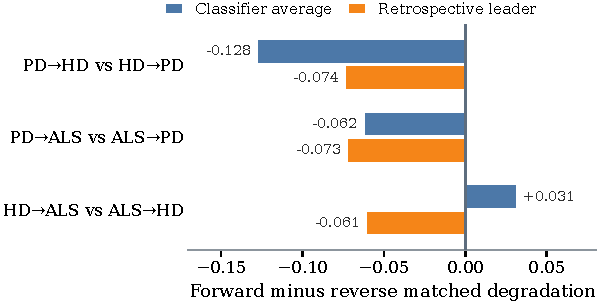
\includegraphics[width=\columnwidth]{figures/arxiv/transfer_asymmetry.pdf}
\caption{Directional asymmetry for each disease pair, measured as matched degradation in the listed forward direction minus that in the reverse direction. Negative values mean the forward direction degraded less. The two bars use different direction summaries: the unweighted classifier average and the retrospective leader. They agree for the two pairs involving PD and disagree for HD and ALS.}
\label{fig:asymmetry}
\end{figure}

Transfer was asymmetric, but the direction of the asymmetry depends on the summary (Fig.~\ref{fig:asymmetry}). Averaged over families, PD~$\rightarrow$~HD degraded 0.1277 less than HD~$\rightarrow$~PD, PD~$\rightarrow$~ALS degraded 0.0625 less than ALS~$\rightarrow$~PD, and ALS~$\rightarrow$~HD degraded 0.0315 less than HD~$\rightarrow$~ALS. The retrospective leaders agree for the two pairs involving PD but reverse the HD and ALS comparison, where the HD~$\rightarrow$~ALS leader degraded 0.0609 less than the ALS~$\rightarrow$~HD leader. Portability depends on the ordered pair, and for HD and ALS it also depends on whether a typical family or the best observed family is considered.

\begin{figure*}[t]
\centering
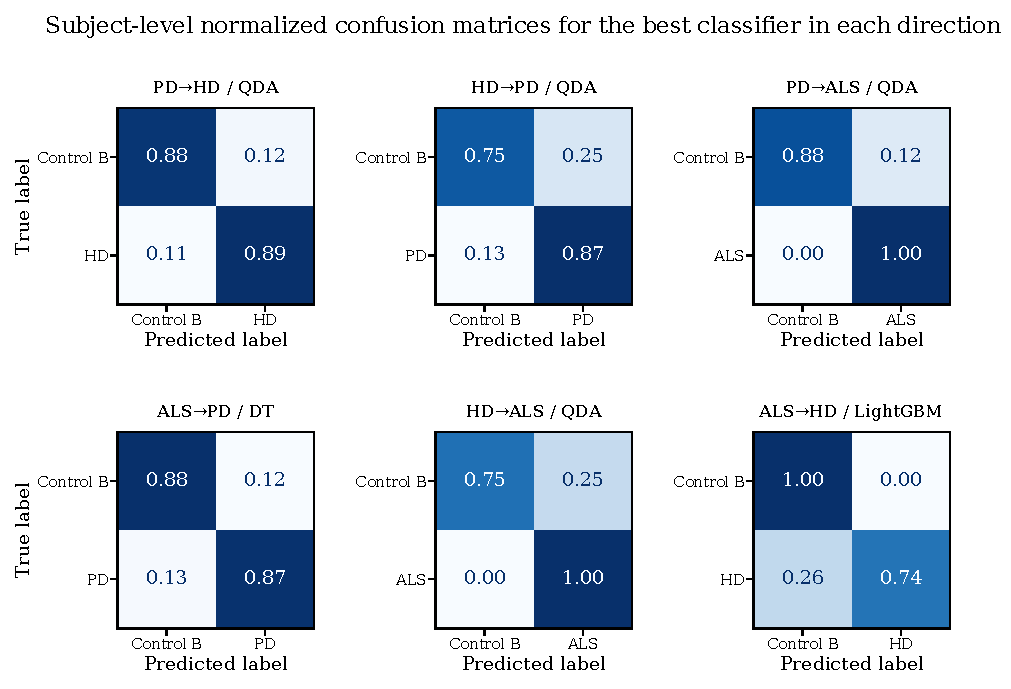
\includegraphics[width=\textwidth]{figures/v4/pdf/step3/step3_subject_confusion_matrices.pdf}
\caption{Subject-level confusion matrices, normalised by true class, for the retrospective leader in each direction. The healthy row is scored on Control~B and the disease row on the target cohort. Leaders were identified after observing target performance.}
\label{fig:confusion}
\end{figure*}

The leaders' errors fall on different sides of the comparison in different directions (Fig.~\ref{fig:confusion}). Quadratic discriminant analysis kept perfect target recall on PD~$\rightarrow$~ALS and HD~$\rightarrow$~ALS, with Control~B specificity of 0.8750 and 0.7500, so those two transfers lost accuracy on the unseen healthy subjects. ALS~$\rightarrow$~HD showed the opposite trade-off, with perfect specificity and a recall of 0.7368. The remaining three leaders made errors on both sides. Six leaders are too few to support a general statement about which error type transfer preserves.

Subject-level uncertainty is large. The per-pair permutation tests, which assess discrimination and not whether matched degradation differs from zero, gave $p<0.05$ for 33 of the 42 pairs, and one pair reached the Monte Carlo floor of $1/10{,}001$. These tests are unadjusted and dependent through the reused Control~B pool, so we treat them as supplementary. The subject-level bootstrap intervals are wide, with a mean 95\% width of 0.2913 for the six retrospective leaders and a median width of 0.3623 across all 42 pairs. Each target evaluation pool contains 21 to 27 subjects, made up of 13 to 19 disease subjects and eight Control~B subjects, so one subject changes a score appreciably and directions that sit close together should not be separated on rank alone.

\subsection{Reliance Shift Under Transfer}
\label{sec:res-shap}

\begin{table}[t]
\caption{Features most often among the three largest raw reliance shifts $\delta_j$ across the 42 classifier-direction pairs.}
\label{tab:recurrence}
\centering
\footnotesize
\begin{tabular}{lcc}
\toprule
Feature & Top-three count & Family \\
\midrule
Stride-time coefficient of variation & 33 & variability \\
Swing-time coefficient of variation & 21 & variability \\
Detrended fluctuation exponent & 19 & fractal \\
Right stride time & 14 & raw timing \\
Left stride time & 11 & raw timing \\
\bottomrule
\end{tabular}
\end{table}

\begin{figure}[t]
\centering
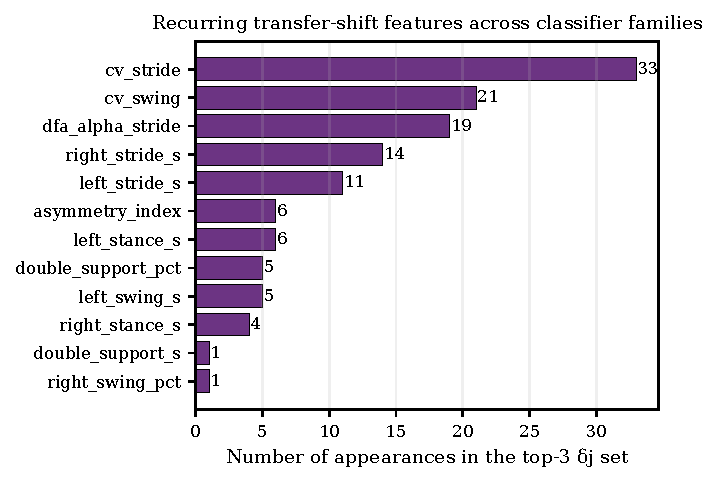
\includegraphics[width=\columnwidth]{figures/v4/pdf/step4/step4_top_feature_recurrence.pdf}
\caption{Number of classifier-direction pairs, out of 42, in which each feature is among the three largest raw shifts $\delta_j$. Bars are coloured by feature family.}
\label{fig:recurrence}
\end{figure}

Table~\ref{tab:recurrence} and Fig.~\ref{fig:recurrence} count how often each feature is among the three largest raw shifts $\delta_j$. The stride-time coefficient of variation appears in 33 of the 42 pairs, followed by the swing-time coefficient of variation (21), the detrended fluctuation exponent (19), and right and left stride time (14 and 11). No other feature appears more than six times. Raw shifts favour features on which a model already relies heavily. When each shift is divided by the within-source reliance on that feature, the most frequent top-three features become right and left stride time and the asymmetry index instead. Which feature looks most displaced depends on how the shift is scaled, and no single feature dominates under both.

\begin{figure*}[t]
\centering
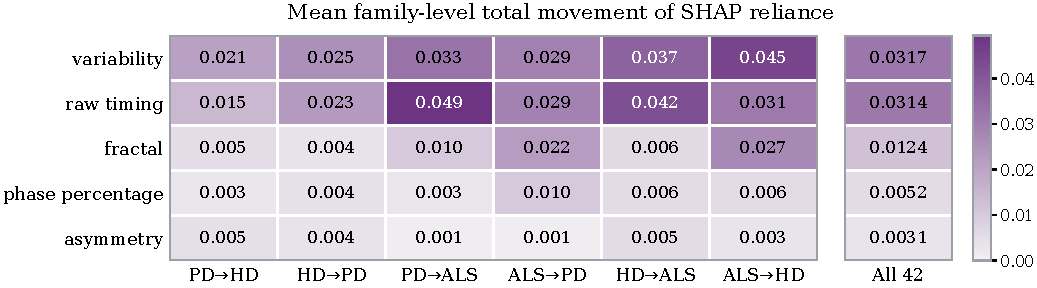
\includegraphics[width=0.9\textwidth]{figures/arxiv/family_movement.pdf}
\caption{Mean family-level total movement of SHAP reliance for each transfer direction, averaged over the seven classifier families, with the average over all 42 pairs on the right. Total movement sums the absolute feature-level changes in mean absolute SHAP magnitude within a family, so opposing movements inside a family do not cancel.}
\label{fig:family-movement}
\end{figure*}

Aggregating by family gives a more stable picture (Fig.~\ref{fig:family-movement}). Measured by total movement, variability (0.0317) and raw timing (0.0314) are effectively tied at the top, followed by fractal structure (0.0124), phase percentage (0.0052), and asymmetry (0.0031). The source condition changes the balance between them. In the two ALS-source directions variability has the largest mean movement (0.0372), and fractal movement (0.0248) is three to five times its value in the PD-source (0.0077) and HD-source (0.0049) directions. In the PD- and HD-source directions raw timing slightly exceeds variability, at 0.0320 against 0.0268 and 0.0324 against 0.0310. The largest single cell is raw timing for PD~$\rightarrow$~ALS.

\begin{figure*}[t]
\centering
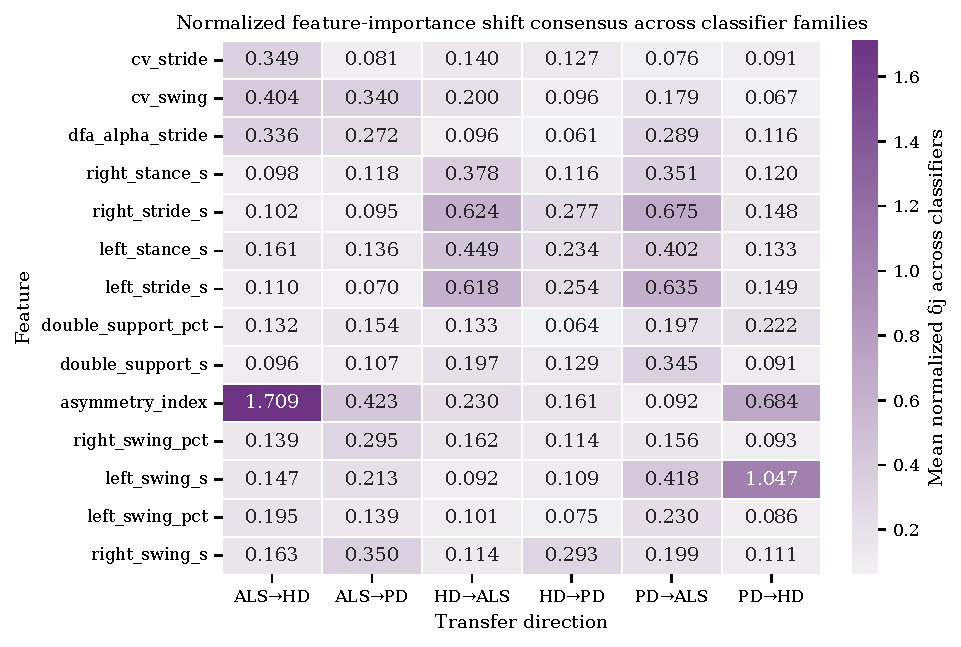
\includegraphics[width=\textwidth]{figures/v4/pdf/step4/step4_delta_j_normalized_consensus_heatmap.pdf}
\caption{Normalised reliance shift $\widetilde{\delta}_j$ for each feature and transfer direction, averaged over the seven classifier families.}
\label{fig:consensus}
\end{figure*}

\begin{figure*}[t]
\centering
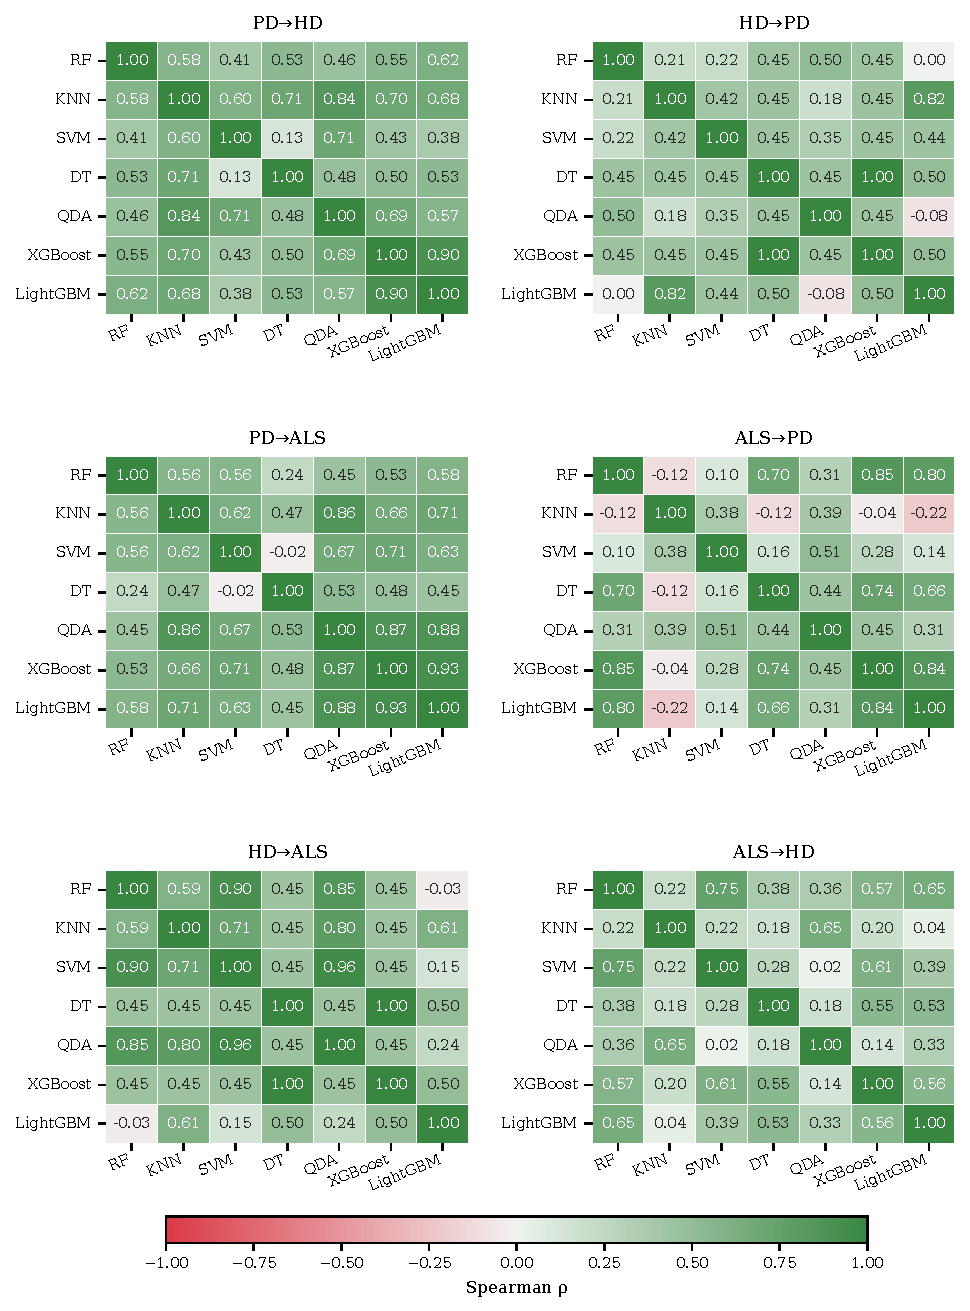
\includegraphics[width=\textwidth]{figures/v4/pdf/step4/step4_delta_j_spearman.pdf}
\caption{Agreement between classifier families on the ranking of reliance shifts, for each transfer direction. Each panel shows the strict lower triangle of a symmetric $7\times7$ Spearman correlation matrix, so the unit diagonal and the mirrored upper half are omitted. Leading zeros are suppressed, so $.58$ denotes $\rho=0.58$. The annotation in each panel gives the median of its 21 distinct classifier pairs.}
\label{fig:spearman}
\end{figure*}

Figs.~\ref{fig:consensus} and~\ref{fig:spearman} show how far the families share these shifts. After averaging over families, the largest normalised shifts belong to the asymmetry index on ALS~$\rightarrow$~HD and to left swing time on PD~$\rightarrow$~HD, and the stride times stand out in the two directions with ALS as the target. The variability descriptors, which dominate the raw counts, are comparatively modest on this scale. The per-direction median rank correlation between families lies between 0.36 and 0.58, so the families share part of their reliance-shift ranking but not most of it, and the degree of agreement depends on the direction. For this reason we read family-level summaries as the more reliable result and treat any single classifier's feature ordering as one view among several.

Reliance movement was only weakly related to transfer cost. Across the 42 pairs, the correlation between the largest normalised shift and matched degradation was Spearman $\rho \approx -0.204$ and Pearson $r \approx -0.042$. The models whose reliance moved most were not the models that lost most accuracy.

\subsection{Dependence on the Control Partition}
\label{sec:res-partition}

\begin{figure}[t]
\centering
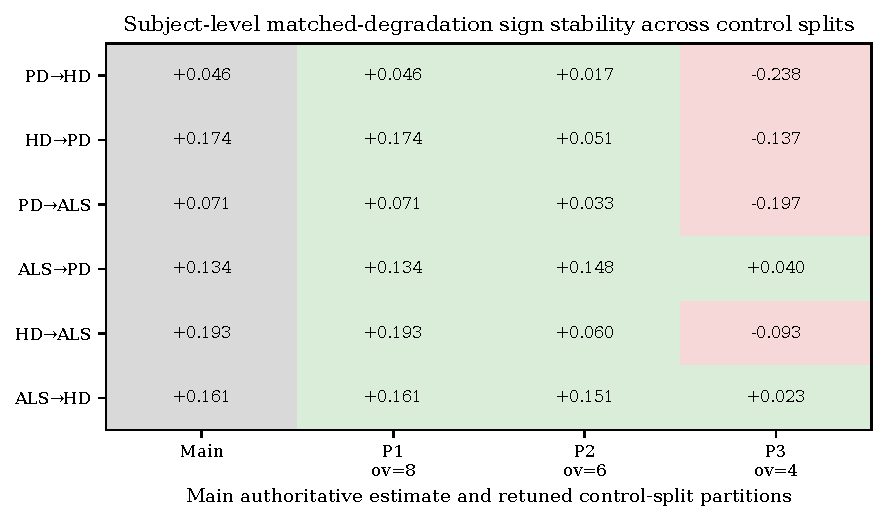
\includegraphics[width=\columnwidth]{figures/v4/pdf/step8/step8_sign_stability_matrix.pdf}
\caption{Direction-level mean matched degradation under the main control partition (P1) and two alternate balanced partitions. The fractions give each partition's overlap with the main Control~A group. P2 preserves all six main-partition signs, and P3 reverses four.}
\label{fig:sign-stability}
\end{figure}

\begin{figure*}[t]
\centering
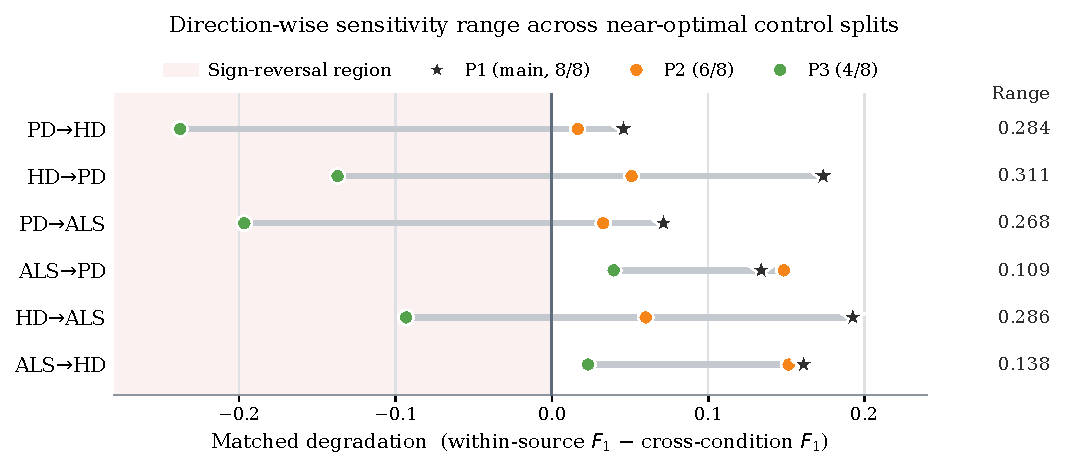
\includegraphics[width=0.9\textwidth]{figures/v4/pdf/step8/step8_direction_degradation_ranges.pdf}
\caption{Range of direction-level mean matched degradation across the three control partitions. A range that crosses into the shaded region belongs to a direction whose sign reverses under some partition. The right-hand column gives each range width.}
\label{fig:ranges}
\end{figure*}

The healthy pools contain only eight subjects each and enter every task, so we repeated the complete within-condition and transfer protocol under two alternate partitions. All three partitions have the same age and gait-speed balance score, and they share eight (P1), six (P2), and four (P3) Control~A subjects with the main split. Each partition is compared against its own within-condition baselines.

Under P2 all six direction means stayed positive, but five of them became smaller (Fig.~\ref{fig:sign-stability}). PD~$\rightarrow$~HD fell from $+0.0458$ to $+0.0165$ and HD~$\rightarrow$~ALS from $+0.1925$ to $+0.0601$, while ALS~$\rightarrow$~PD rose slightly to $+0.1484$. Under P3 four directions reversed sign: PD~$\rightarrow$~HD reached $-0.2378$, HD~$\rightarrow$~PD $-0.1371$, PD~$\rightarrow$~ALS $-0.1967$, and HD~$\rightarrow$~ALS $-0.0932$. Only the ALS-source directions stayed positive, at $+0.0396$ for ALS~$\rightarrow$~PD and $+0.0231$ for ALS~$\rightarrow$~HD. Sign agreement with the main partition was six of six for P2 and two of six for P3, and the rank correlation of the six direction means with the main ordering was 0.543 and 0.486.

Because matched degradation subtracts a cross-condition score from a within-condition score, a partition can change it from either side. Under P3 most of the change came from the within-condition side. Averaged over families, the within-condition estimate fell from 0.8736 to 0.6288 for PD, from 0.8738 to 0.6899 for HD, and from 0.9259 to 0.8262 for ALS, while the cross-condition means changed by between $-0.0055$ and $+0.1267$. With a different Control~A group the source tasks themselves became harder to separate, and the matched degradation inherited that change.

The ranges across partitions (Fig.~\ref{fig:ranges}) run from 0.1088 for ALS~$\rightarrow$~PD to 0.3106 for HD~$\rightarrow$~PD. In four directions the range is larger than the entire spread of direction means under the main partition, which is 0.1467.

\subsection{Stride-Level Robustness Diagnostics}
\label{sec:res-robust}
The diagnostics in this subsection score stride rows directly, without subject aggregation, so they are reported as stride-level macro-$F_1$ and are not comparable with the subject-level results above. Within-condition analyses replay the saved outer-fold models, and transfer analyses use the saved full-source models.

\begin{figure*}[t]
\centering
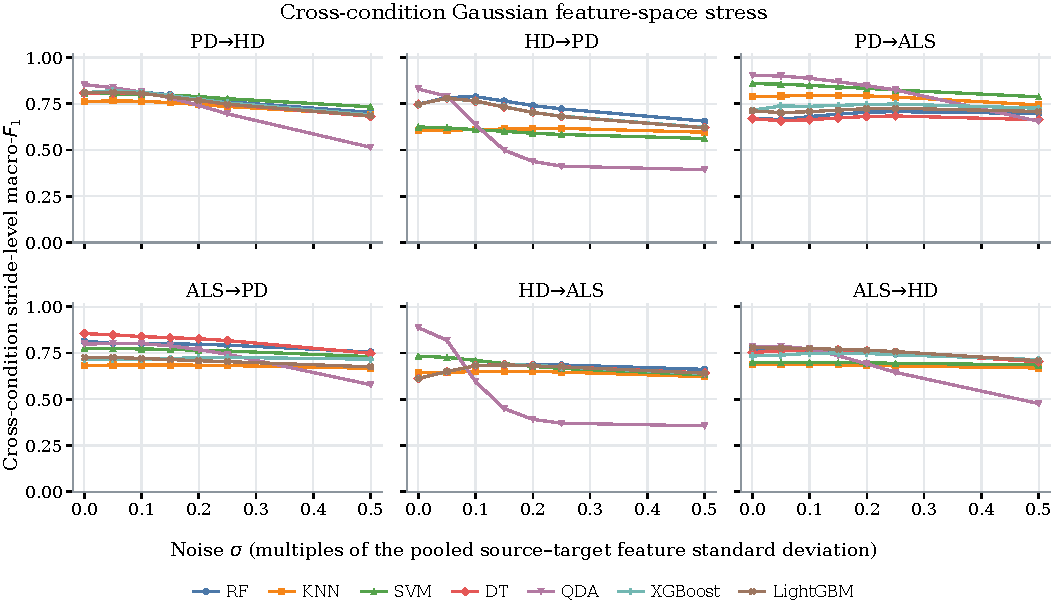
\includegraphics[width=\textwidth]{figures/arxiv/noise_curves_cross.pdf}
\caption{Cross-condition stride-level macro-$F_1$ under Gaussian feature-space noise, for every classifier family and transfer direction. Noise is scaled by the standard deviation of each feature over the pooled source and target rows, and each point averages 30 repetitions. Quadratic discriminant analysis declines most steeply in every direction, and most of all in the two HD-source directions.}
\label{fig:noise}
\end{figure*}

\textit{Gaussian stress.} Fig.~\ref{fig:noise} shows stride-level macro-$F_1$ as Gaussian noise is added to the engineered features of the target pool. Each value averages the seven classifiers and 30 repetitions. Without noise the direction means ranged from 0.6732 for HD~$\rightarrow$~ALS to 0.8077 for PD~$\rightarrow$~HD. At $\sigma = 0.50$ the two HD-source directions were the lowest, at 0.5818 for HD~$\rightarrow$~PD and 0.5992 for HD~$\rightarrow$~ALS, as they had been without noise. PD~$\rightarrow$~ALS retained 0.7119, ALS~$\rightarrow$~PD 0.6960, PD~$\rightarrow$~HD 0.6715, and ALS~$\rightarrow$~HD 0.6661. The largest declines were in PD~$\rightarrow$~HD and HD~$\rightarrow$~PD, about 0.14 each, and the smallest was in PD~$\rightarrow$~ALS, about 0.05. Quadratic discriminant analysis declined most steeply in every direction, from 0.83 to 0.39 on HD~$\rightarrow$~PD and from 0.89 to 0.36 on HD~$\rightarrow$~ALS. The tree-based models changed little, and on HD~$\rightarrow$~ALS several of them improved slightly. Within condition, where noise is scaled by the feature standard deviations of the source pool, the classifier-averaged stride-level score fell from 0.8729 to 0.7485 for PD, from 0.8782 to 0.6599 for HD, and from 0.8854 to 0.7921 for ALS.

\begin{figure}[t]
\centering
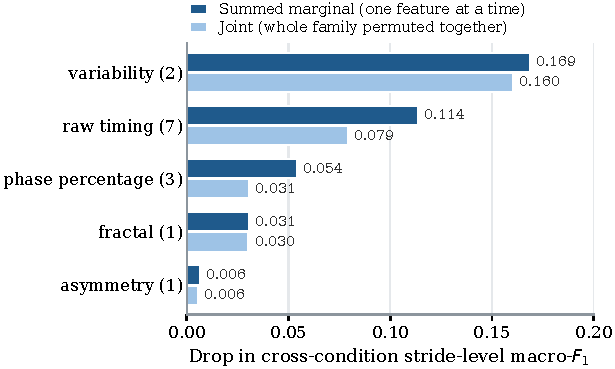
\includegraphics[width=\columnwidth]{figures/arxiv/family_sensitivity.pdf}
\caption{Cross-condition permutation sensitivity by feature family, as the drop in stride-level macro-$F_1$ averaged over the 42 classifier-direction pairs. The dark bars sum the drops from permuting each feature on its own; the light bars permute the whole family together. The number of features in each family is given in parentheses. Within-condition values are omitted because permutation there cannot move the subject-level descriptors (Section~\ref{sec:res-robust}).}
\label{fig:family-sensitivity}
\end{figure}

\textit{Permutation sensitivity.} Fig.~\ref{fig:family-sensitivity} reports how much the transferred models depend on each family. Features were first permuted one at a time and the resulting drops summed within each family. On this basis the drop was largest for variability (0.1685) and raw timing (0.1137), followed by phase percentage (0.0541), fractal structure (0.0307), and asymmetry (0.0063). Permuting all features of a family together with one shared row order gave 0.1605, 0.0790, 0.0306, 0.0303, and 0.0056, so the same two families remain at the top. The joint drop is noticeably smaller than the summed drop only for the multi-feature raw timing and phase percentage families, which is consistent with overlapping information among their features. These values should be read with two caveats. The families differ in size, and permuting stride rows in a target pool that contains many subjects moves the subject-level descriptors between subjects. What these values measure is representation-specific aggregate model sensitivity, not intrinsic family importance. Within-condition permutation behaves differently for a structural reason. Rows are shuffled inside each held-out subject, where the two coefficients of variation and the fluctuation exponent are constant, so their within-condition drops are exactly zero by construction. The within-condition drops for raw timing (0.0053) and phase percentage (0.0198) cannot be compared with the cross-condition values for the same reason, and we do not interpret the within-versus-cross contrast.

\textit{Structured corruption.} Under the heaviest setting of each corruption type, and again on stride-level macro-$F_1$, label corruption was the most damaging at 0.6384, followed by Gaussian jitter at 0.6624 and gain and bias drift at 0.6874, with feature masking at 0.7205 and row dropout at 0.7453 the least damaging. Each value averages the six directions and seven classifiers, and the jitter and gain-and-bias values additionally average their three recorded scaling variants. Label corruption flips the evaluation labels themselves, so its effect measures how sensitive the metric is to annotation errors and not how the model degrades. The other perturbations act on the engineered features and on the evaluation table and are stress tests of the fitted models, not simulations of sensor failure.

\textit{Per-subject sensitivity.} The stride-level accuracy of individual target subjects is highly uneven. Across all 42 pairs its median is 1.0, but about one subject-pair entry in five falls below 0.5. Each retrospective leader classified between one and five target subjects correctly on fewer than half of their strides. Transfer errors are concentrated in a minority of subjects and are not spread evenly across the target pool.

\subsection{Exploratory Subject-Level Geometry}
\label{sec:res-geometry}

\begin{figure*}[t]
\centering
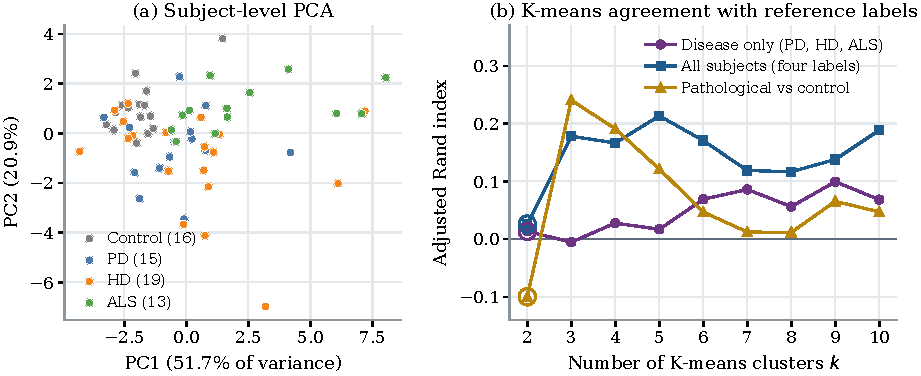
\includegraphics[width=\textwidth]{figures/arxiv/subject_geometry.pdf}
\caption{Exploratory subject-level geometry of the engineered features. (a) First two principal components of the 63 subjects, after averaging stride features within each subject and z-scoring across subjects. (b) Adjusted Rand index between K-means clusters and the reference labels of three views, for $k=2$ to $10$. Rings mark the $k$ selected by the silhouette criterion, which is $k=2$ in every view.}
\label{fig:geometry}
\end{figure*}

As descriptive context, Fig.~\ref{fig:geometry} summarises the subject-level feature space. The first two principal components explain 72.6\% of the variance across all 63 subjects (51.7\% and 20.9\%) and 69.9\% across the 47 patients alone. PD subjects overlap substantially with the healthy controls, whereas several HD and ALS subjects lie far along the first component.

K-means clustering does not recover the diagnostic labels. The silhouette criterion selects $k=2$ in every view, and at that $k$ the adjusted Rand index is 0.0135 for the patients alone, 0.0260 for all subjects with four labels, and $-0.0999$ for pathological against control. In the two-cluster solution all 16 controls share a cluster with 38 of the 47 patients, and the second cluster holds nine patients, five of whom have ALS. Larger values of $k$ raise the agreement to at most 0.2404 (pathological against control, $k=3$), 0.2134 (all subjects, $k=5$), and 0.0993 (patients only, $k=9$). The clusterings are stable across random seeds, with a mean adjusted Rand index of 0.98 for all subjects, but unstable under subject resampling, where it falls to 0.04. In this representation the dominant unsupervised structure separates a small group of atypical patients, mostly with ALS, from everyone else. We use this view as context only and draw no conclusion about transferability from it.

\section{Discussion}
\label{sec:discussion}

\subsection{What the Benchmark Supports}
Under the main control partition, every classifier-averaged direction summary retained subject-level macro-$F_1$ between 0.6812 and 0.8278, and every one of them fell below its matched within-source baseline. Individual models were less uniform. Seven of the 42 classifier-direction pairs scored above their own within-condition estimate, and the retrospective leader did so in four of the six directions. The benchmark therefore supports two statements together: a boundary learned on one neurological condition carries measurable information about another, and on average it carries less than it did within its own condition.

The limits of that conclusion are equally specific. The pairs that transferred without loss were identified after the target labels had been scored, so they describe the best observed outcome among the seven families we evaluated. They do not show that such a model could have been chosen in advance, and they say nothing about classifiers outside that set. The classifier averages have a similar scope. They are unweighted means over seven families chosen for this study, so they summarise this benchmark and are not estimates for classifiers in general.

\subsection{Within-Condition Accuracy and Portability}
Strong source performance did not predict strong transfer. HD produced the second strongest within-condition leader, yet the two HD-source directions had the lowest mean subject-level macro-$F_1$ (0.7003 and 0.6812) and the largest mean degradation. Model families showed the same pattern. Quadratic discriminant analysis led only the ALS source task but was the retrospective leader in four directions. The decision tree that led PD was the leader only for ALS~$\rightarrow$~PD, and XGBoost, which led HD, did not lead any direction.

One property of the task makes this less surprising. Transfer changes the disease cohort and the healthy pool at the same time, so a boundary can lose accuracy on either side of the comparison, and the retrospective leaders show both cases. Two of them kept perfect target recall while losing specificity on Control~B, whereas the ALS~$\rightarrow$~HD leader kept perfect specificity and missed HD subjects. Directional asymmetry is also less stable than the direction means alone suggest. The classifier averages and the retrospective leaders agree that PD-source transfer degraded less than its reverse, but they disagree about the HD and ALS pair.

We record these orderings without explaining them. With seven families, three source pools, and eight controls on each side, the design cannot isolate why one family transfers better than another, and classifier-family effects here should not be read as statements about gait physiology.

\subsection{What the Diagnostics Add}
The reliance-shift and permutation analyses both placed the largest aggregate diagnostic burden on variability and raw timing, and permuting whole families jointly kept the same two families at the top. The agreement is useful, but three properties limit what it shows. Both analyses use the same fitted models and the same target rows, so they are complementary rather than independent evidence. Both sum over families of unequal size, and raw timing has seven features against two for variability. Stride-level permutation in a multi-subject target pool also moves the broadcast subject-level descriptors across subjects, which creates feature combinations that no recorded subject had. The results describe how these fitted models respond to this particular representation. They do not rank the intrinsic importance of gait timing families, and neither analysis supports a causal reading.

The association between reliance movement and transfer cost was weak (Spearman $\rho \approx -0.204$). A model can keep its score while its reliance profile moves, or lose accuracy while its most displaced feature changes little, so the two quantities are best reported as separate properties of a transfer.

The stride-level stress tests contribute a different kind of information. The HD-source directions were already the weakest before any noise was added and remained so under the largest perturbation, which means the stress preserved an existing ordering rather than creating one. Quadratic discriminant analysis, the family that led most directions retrospectively, also declined most steeply under Gaussian noise in every direction. We note this co-occurrence without claiming that one property explains the other.

\subsection{The Control Partition as an Experimental Factor}
The three partitions share the same age and gait-speed balance score, so neither alternate is a less balanced version of the main split. Even so, the partition sharing six of eight Control~A subjects with the main split preserved all six positive direction signs, while the partition sharing four of eight reversed four of them. Only the two ALS-source directions stayed positive under all three. In four directions the range across partitions was larger than the entire spread of direction means under the main partition. The decomposition in Section~\ref{sec:res-partition} shows that the largest changes came from the within-condition side: with a different Control~A group the PD and HD source tasks became much harder to separate, so the reversals reflect lower matched baselines more than better transfer. Matched degradation depends on both terms of its subtraction, and the healthy subjects assigned to the source pool affect it as strongly as those assigned to the target pool. With eight healthy subjects on each side, the assignment of individual controls moved the transfer estimate by as much as the choice of direction did. We therefore treat the main-partition signs as a property of that partition and report the disagreement between partitions instead of averaging over them.

\subsection{Limitations}
The cohort is small in the unit that matters. It contains 15 PD, 19 HD, 13 ALS, and 16 control subjects, and each target evaluation pool contains between 21 and 27 subjects, so one subject can change a score appreciably. The large number of stride rows does not reduce this subject-level uncertainty. The benchmark also uses a single public dataset and has no external validation cohort.

Control~A and Control~B are balanced with each other on age and gait speed. This balance does not make either control group demographically comparable to the disease cohorts, so part of every abnormal-versus-control boundary may reflect age, gait speed, or other differences between patients and controls instead of disease-related gait.

The representation is deliberately narrow. It covers engineered stride timing only and excludes force waveforms, spatial kinematics, wearable signals, medication state, and disease severity. Within it, the raw timing variables are mechanically linked, the phase percentages are compositional, and three descriptors are subject-level values repeated on every stride. The detrended fluctuation exponent is computed from a stride series from which filtered rows have been removed, so it is a pragmatic descriptor and not a complete measure of fractal gait dynamics.

The inferential scope is limited as well. The permutation tests assess discrimination for each classifier-direction pair. They are unadjusted, they are dependent through the reused Control~B pool, and they do not test whether matched degradation differs from zero. No direction-level hypothesis test was performed. The bootstrap intervals resample completed subject predictions and are conditional on the fitted source models, so they do not propagate uncertainty from hyperparameter selection or source training. The classifier set and its grids were fixed in advance, and a different set of families would give different averages and could give different leaders.

The diagnostics have their own limits. Attribution over correlated engineered features can divide credit among mechanically linked variables \cite{aas2021dependentshap}, kernel SHAP estimates are approximate and were computed on stratified subsamples, and the robustness perturbations act on engineered features and evaluation tables, not on sensors. The repository also contains an exploratory conformal prediction analysis, which we do not use as evidence. In the transfer setting its calibration scores are computed from the full-source model's predictions on the same rows used to fit that model. The calibration is not held out, the resulting thresholds are optimistic, and the procedure does not provide split-conformal coverage.

\subsection{Future Work}
The most direct extension is a model-selection rule that does not read target labels. Two variants should be kept separate: a source-only rule, which selects a model from source validation alone, and a transductive rule, which is label-free but inspects unlabelled target features. Either would turn the retrospective leaders into an operational procedure, and only the first leaves the target pool untouched.

Larger cohorts with more varied healthy pools are needed to establish whether the partition sensitivity reflects the small sample or the transfer task itself. Richer representations, such as raw timing sequences, force signals, kinematics, or wearable data, would show how much of the degradation is due to the engineered timing features. Domain adaptation and domain generalisation baselines designed for cross-condition domain shift would indicate how much of it can be recovered. Uncertainty statements under this kind of shift would need a held-out calibration design together with methods that account for the difference between source and target distributions \cite{angelopoulos2021conformal,tibshirani2019conformalshift}. Where the metadata allow it, medication state and disease severity should also be examined as sources of variation.

\section{Conclusion}
\label{sec:conclusion}
We asked whether an abnormal-versus-control gait timing boundary learned from one neurological condition remains useful on another. To answer it, we built a leakage-controlled benchmark on PhysioNet GAITNDD with subject-level evaluation, disjoint healthy control pools, and no target labels, retuning, threshold selection, or calibration.

Transfer was measurable, degraded, and asymmetric. Every classifier-averaged direction summary retained non-trivial subject-level discrimination and fell below its matched within-source baseline, while seven individual classifier-direction pairs exceeded their baselines when examined retrospectively. Reliance-shift and permutation diagnostics placed the largest aggregate burden on variability and raw timing, and one alternate balanced control partition reversed four of the six direction-level signs.

For cohorts of this size a single transfer score is not a sufficient summary. Transfer results should state the endpoint and its aggregation unit, keep classifier averages separate from retrospectively selected models, and name the healthy-control partition on which they depend.

\bibliographystyle{IEEEtran}
\bibliography{references}

\end{document}
